\documentclass{article}
\usepackage[russian]{babel}
\usepackage[utf8]{inputenc}
\usepackage{epsfig}
\usepackage{graphicx}
\usepackage{caption}
\usepackage{subcaption}
\usepackage{amssymb}
\usepackage{amsmath}

\title
    {Решение задачи MAP для марковской сети типа решётка}
\author
    {Новиков~А.\,В.\\
    МГУ, ВМиК, каф. ММП}

\begin{document}
\maketitle

\pagebreak

\section{Постановка задачи}
Марковские сети применяются практически повсюду.
После обучение сети нужно её использовать,
то есть решать задачу максимизации апостериорной вероятности.
Для большинства реальных задач эта задача NP--трудная.\\
В данной статье проводится обзор существующих
state-of-the-art подходов к этой задаче.
\pagebreak

\section{Методы}
Мы остановились на подклассе алгоритмов использующих
двойственное разложение. В них задача минимазации
исходной энергии сводится к задаче максимизации
двойственной энергии (это функция всегда выпула вверх).
Алгоритмы этой группы отличает конкретный метод максимизации.
\begin{itemize}
\item Субградиентный подъём~\cite{Subgradient}
\item Bundle methods~\cite{Bundle}
\item <<Полная декомпозиция>>
\end{itemize}
\pagebreak

\section{Данные}
Для сравнения подходов мы использовали данные
опубликованные Karteek Alahari~\cite{Alahari}
\pagebreak


\section{Субградиентный подъём}
Результаты работы данного метода зависят от выбора
последовательности шагов $\alpha_t$.
Использовался константный, адаптивный шаг и неточная
одномерная оптимизация по величине шага.\\
Адаптивный подход нашел глобальный минимум,
показав результат лучше чем $\alpha$--расширение,
но работал примерно в $60$ раз дольше.
Использование константного подхода показывает
примерно одинаковые результаты для разных констант
из хорошего диапазона. Если не угадать с константой,
то метод либо разойдётся, либо будет сходится слишком медленно.
В случае адаптивного шага использовалась следующая формула:\\
$\alpha_t = \frac{Approx_t - Dual_t}{\left \| \Delta \overrightarrow{g_t} \right \|^2}$\\
Где $Dual_t$~--- текущее значение двойственной функции, 
$Approx_t$~--- оценка оптимума двойственной функции.\\
$Approx_t = BestDual_t + \delta_t$,\\
где $BestDual_t$~--- лучшее на данный момент значение двойственной функции,\\
\begin{equation}
    \delta_{t+1} = \begin{cases}
    \gamma_0 \delta_t, & Dual_t > Dual_{t-1},\\
    max(\gamma_1 \delta_t, \epsilon) & Dual_t \leqslant  Dual_{t-1}.
    \end{cases}
\end{equation}
$\gamma_0$, $\gamma_1$, $\epsilon$~--- параметры метода, выбранные нами эмпирически.\\
$\gamma_0 = 1.5$\\
$\gamma_1 = 0.5$\\
$\epsilon_t = \frac{1}{t}$\\


\begin{figure}
    \centering
    \begin{subfigure}[t]{\textwidth}
            \centering
            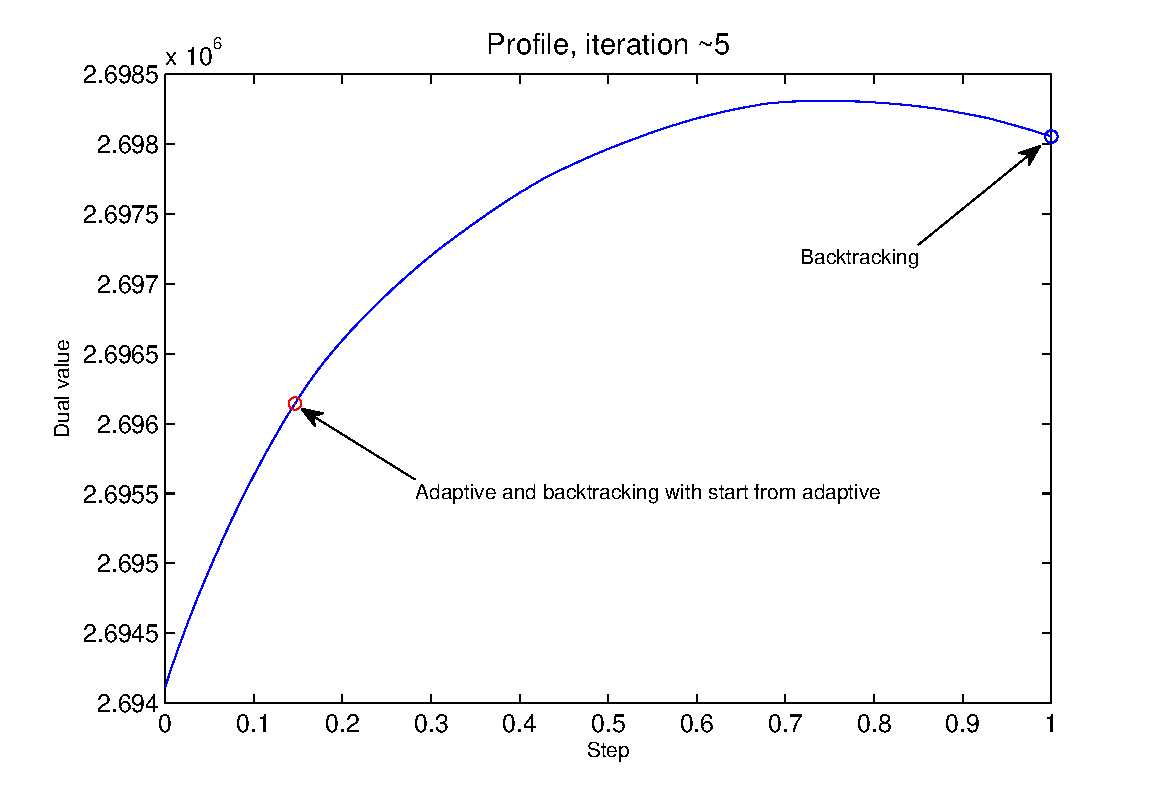
\includegraphics[width=0.9\textwidth]{profile_tsukuba.eps}
    \end{subfigure}
    \begin{subfigure}[t]{\textwidth}
            \centering
            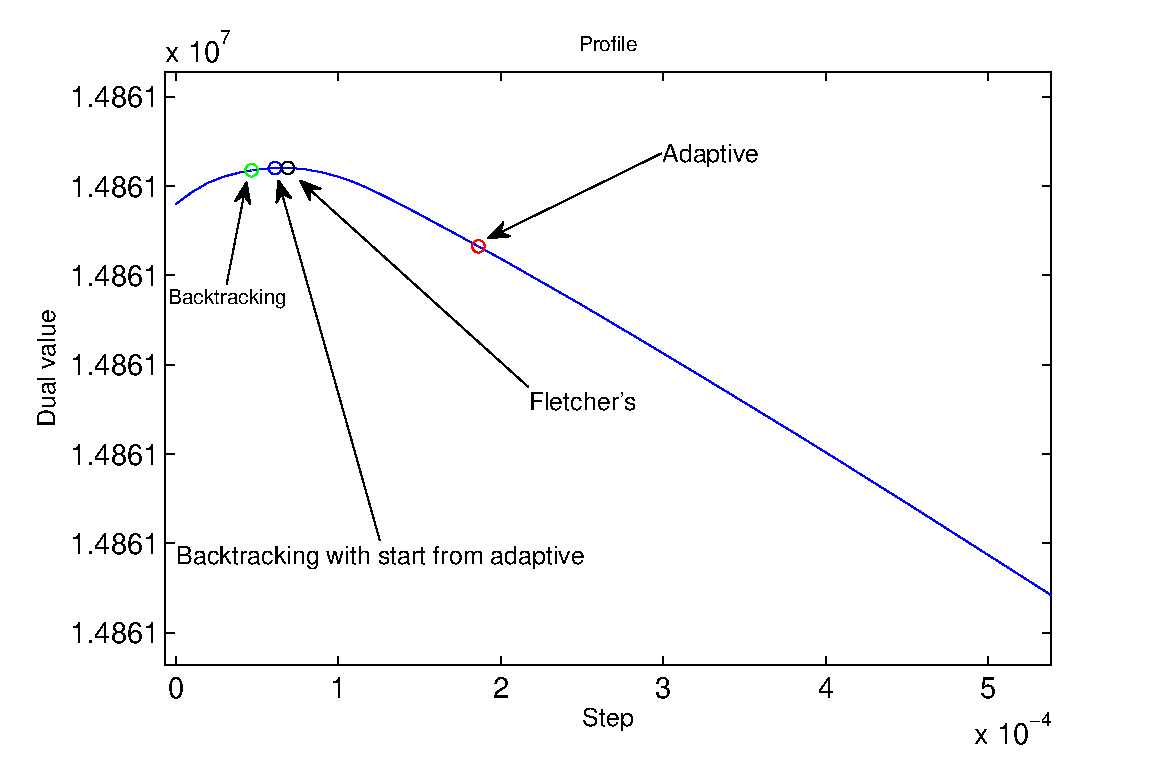
\includegraphics[width=0.9\textwidth]{profile_cones.eps}
    \end{subfigure}
    \caption{Профиль двойственной функции вдоль направления оптимизации и неточные максимумы найденные различными алгоритмами}
    \label{fig:profile}
\end{figure}
Не смотря на то, что двойственная функция является кусочно линейной, она очень близка к гладкой, так что методы неточной одномерной оптимизации кажутся довольно перспективным направлением работы~(рис.~\ref{fig:profile}). Нами был опробован метод Флетчера и <<backtracking>>.\\


На графиках приведены примеры работы алгоритмов (в том числе
длинны шагов, выбранных адаптивным методом) на стереопаре Tsukuba.
\begin{figure}
    \centering
    \begin{subfigure}[t]{\textwidth}
            \centering
            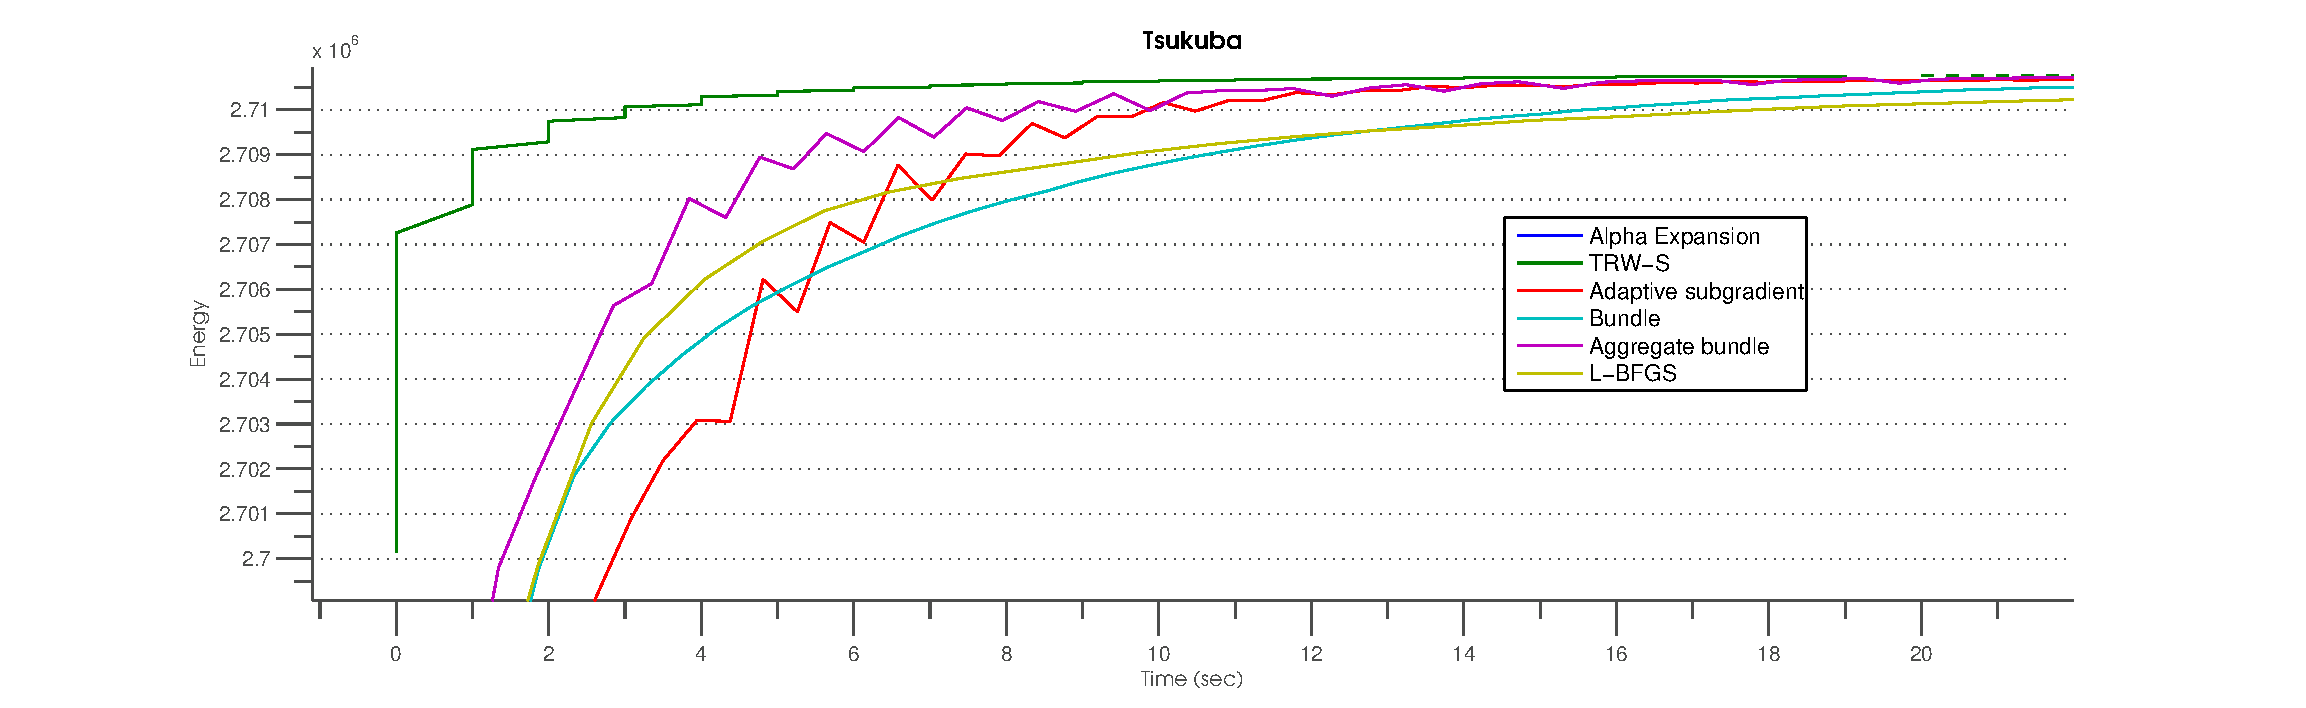
\includegraphics[width=1.5\textwidth]{comparative_tsukuba.eps}
            \caption{Сравнение скорости и качества работы различных методов.
                    Для $\alpha$--расширения указанна только прямая энергия,
                    для остальных алгоритмов указанна прямая и двойственная энергия.}
    \end{subfigure}
    \begin{subfigure}[t]{\textwidth}
            \centering
            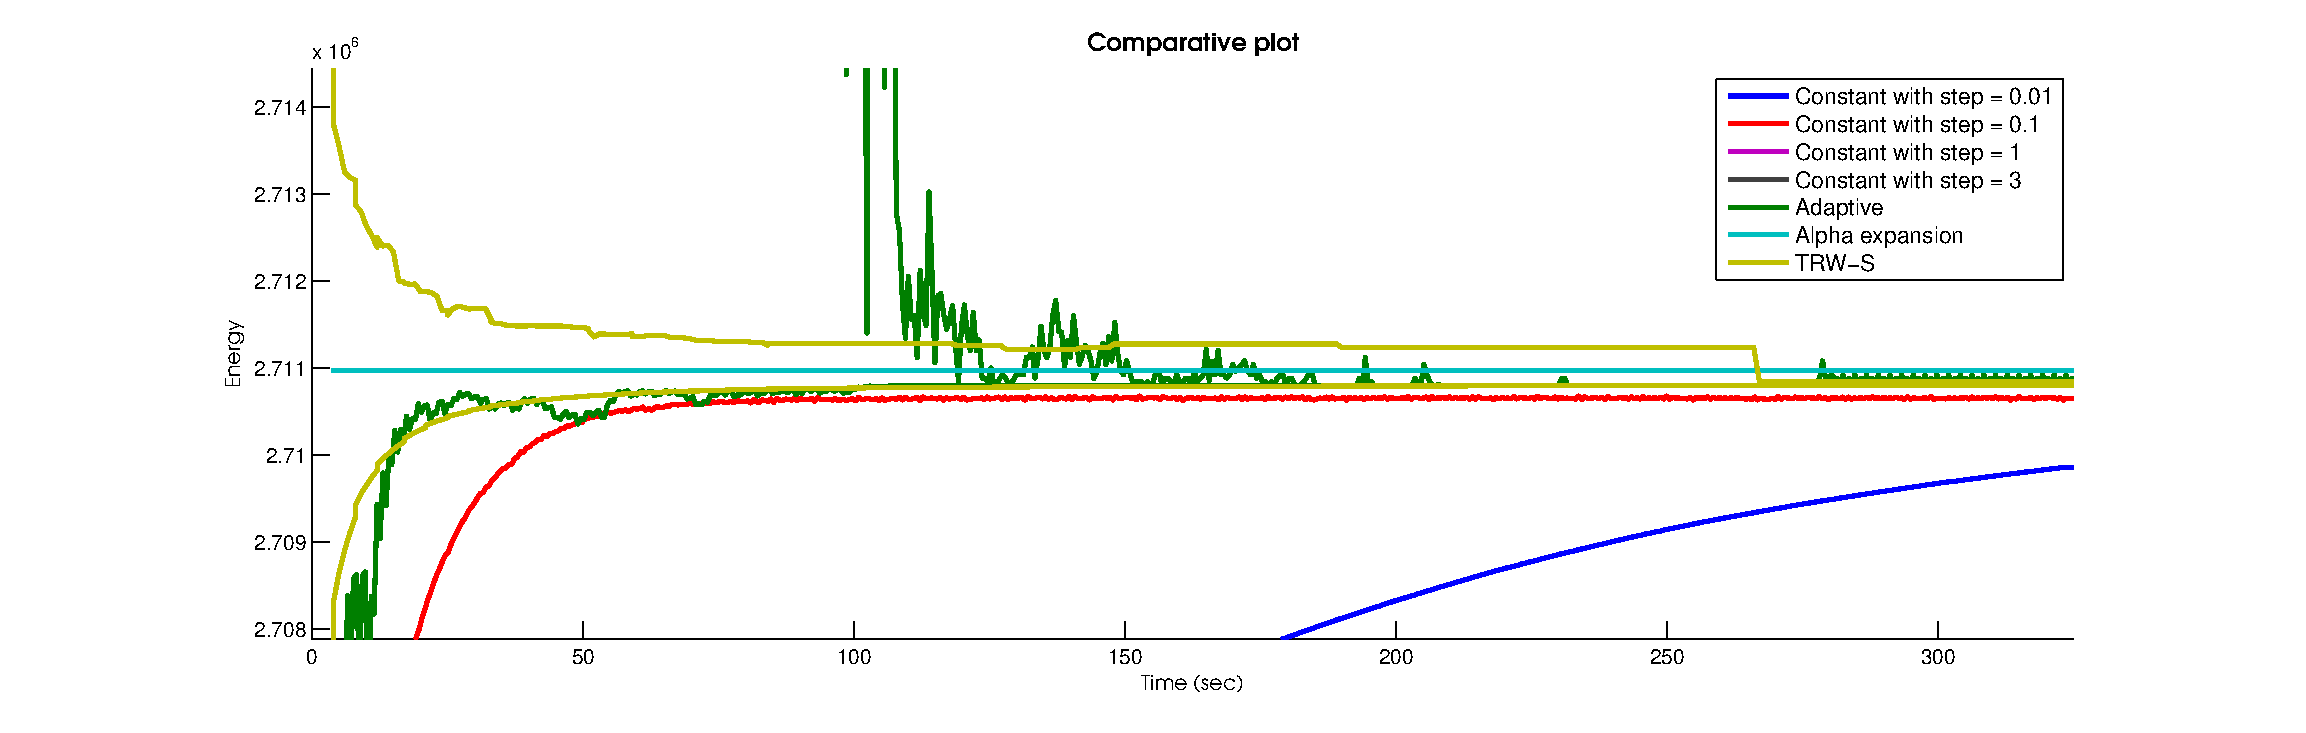
\includegraphics[width=1.5\textwidth]{comparative_tsukuba_small.eps}
    \end{subfigure}
    \begin{subfigure}[t]{\textwidth}
            \centering
            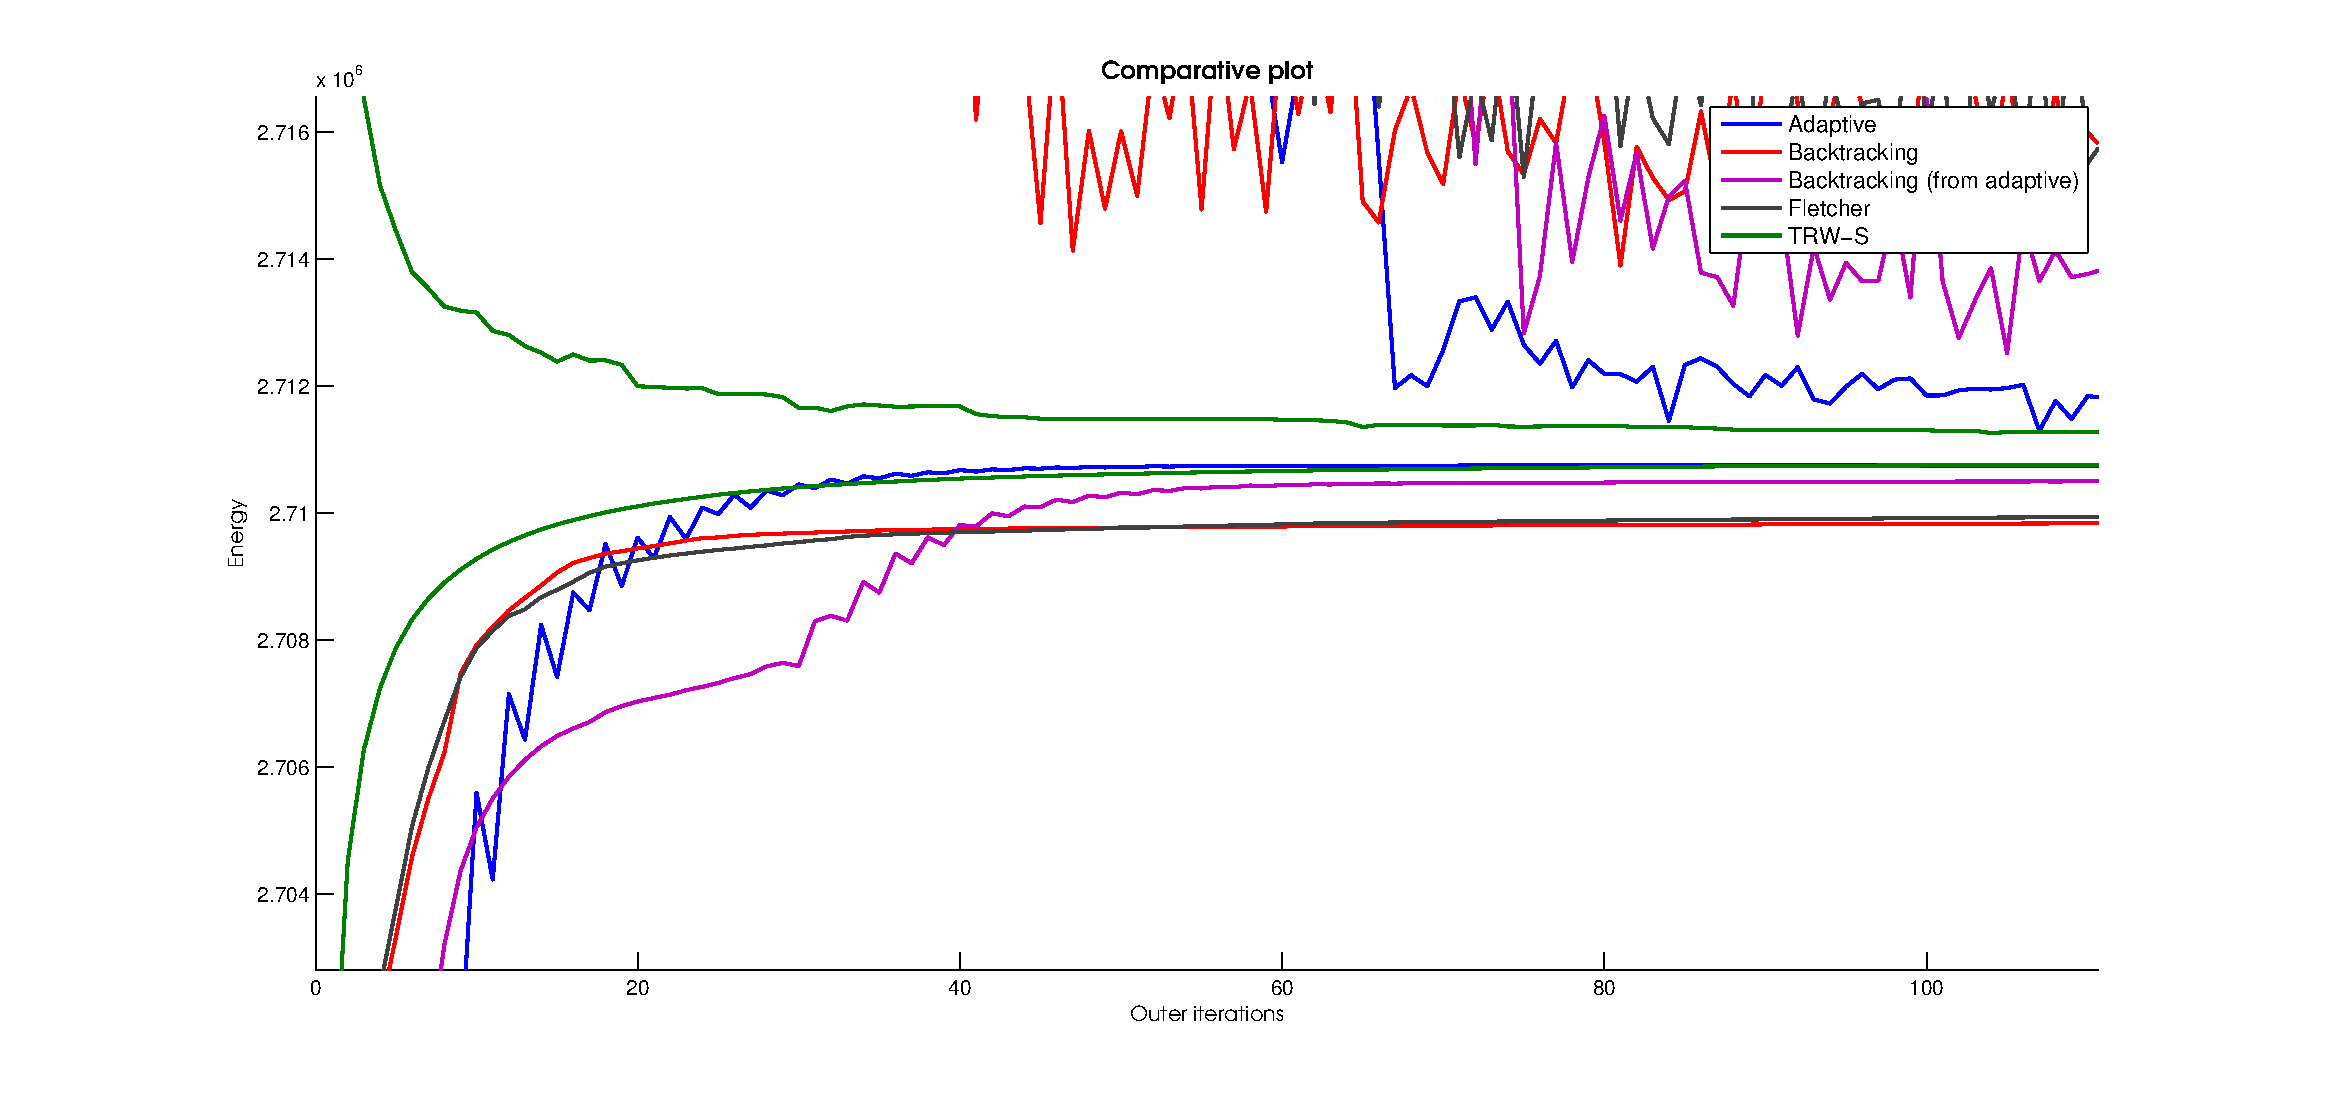
\includegraphics[width=1.5\textwidth]{1d_optimization.eps}
    \end{subfigure}
\end{figure}

\begin{figure}
    \centering
    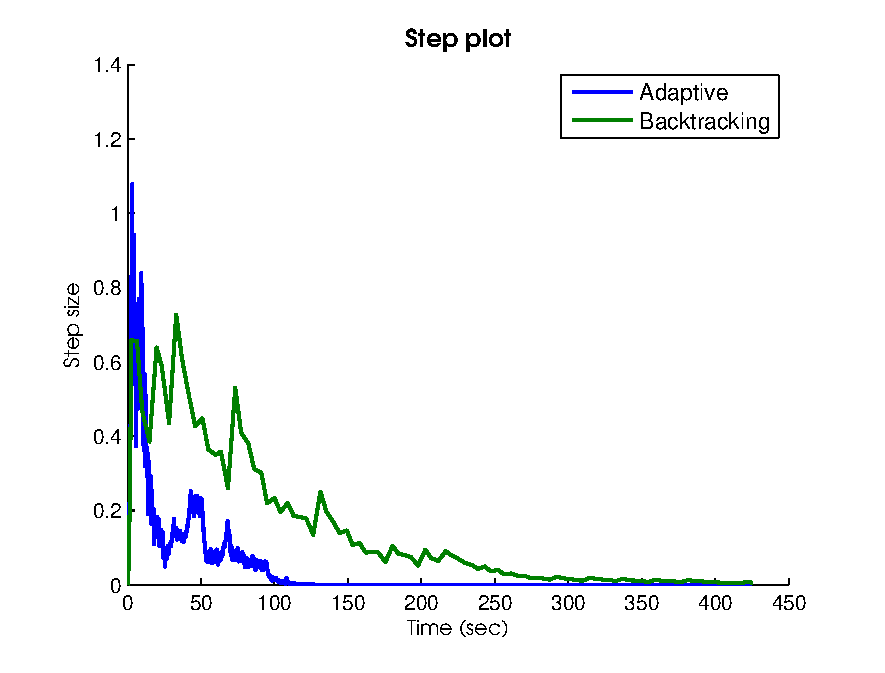
\includegraphics[width=\textwidth]{step_adap_vs_adapBack.eps}
    \caption{Длинна шага выбранная на каждой итерации адаптивным методом и методом <<backtracking>>}
\end{figure}

\begin{figure}
    \centering
    \begin{subfigure}[t]{\textwidth}
            \centering
            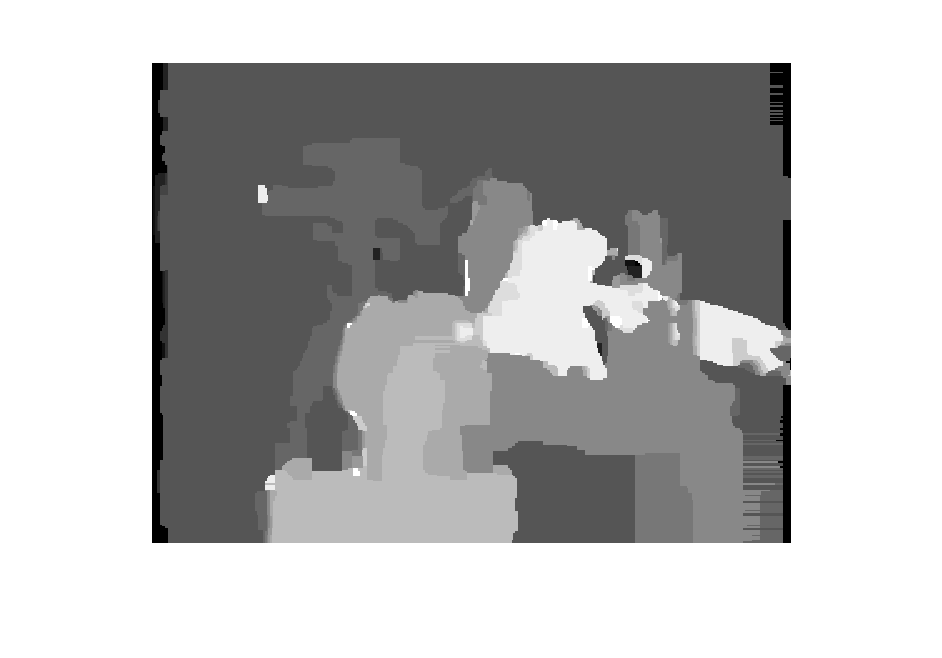
\includegraphics[width=\textwidth]{adaptive_result.eps}
            \caption{Итоговая разметка выбранная наилучшим методом (адаптивным)}
    \end{subfigure}
    \begin{subfigure}[t]{\textwidth}
            \centering
            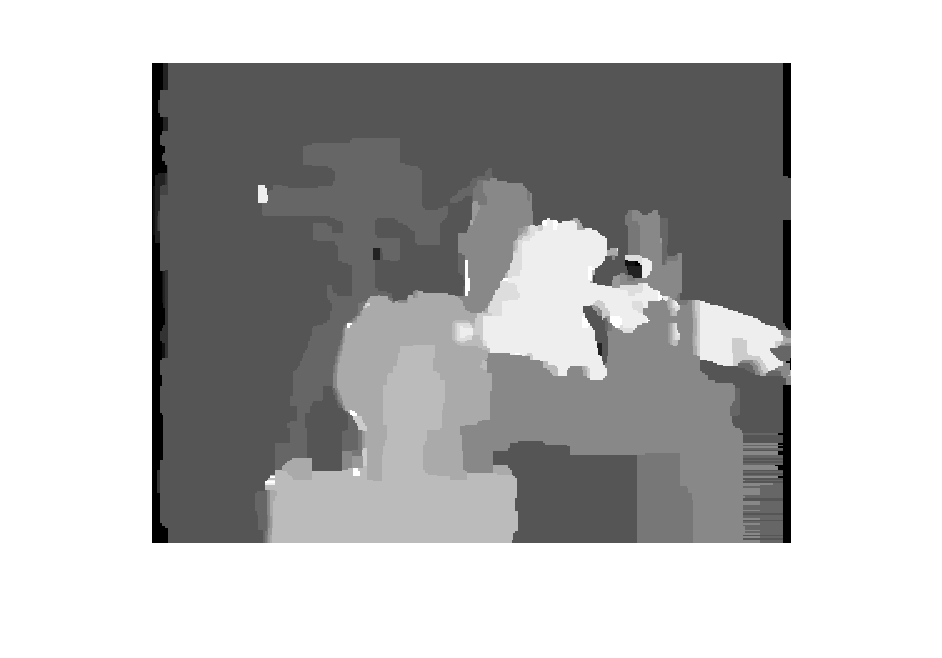
\includegraphics[width=\textwidth]{constant_0_1_result.eps}
            \caption{Разметка выбранная константным методом с длинной шага $0.1$}
    \end{subfigure}
\end{figure}


\begin{thebibliography}{1}
\bibitem{Alahari}
    {Alahari~K., Kohli~P., Torr~P.~H.~S.}
    {Dynamic Hybrid Algorithms for MAP Inference in Discrete MRFs}~//
    {IEEE} Trans. Pattern Anal. Mach. Intell., 2010.~--- С.\,1846--1857.
\bibitem{Subgradient}
    {Komodakis~N., Paragios~N., Tziritas~G.}
    {MRF energy minimization and beyond via dual decomposition}~//
    Pattern Analysis and Machine Intelligence, IEEE Transactions on, 2011.~--- С.\,531--552.
\bibitem{Bundle}
    {Kappes~J.\,H.}
    {A Bundle Approach To Efficient MAP-Inference by Lagrangian Relaxation}~//
    Computer Vision and Pattern Recognition (CVPR), IEEE Conference 2012.~--- С.\,1688--1695.
\end{thebibliography}
\end{document}
